\chapter{Introduction to the SSFM for vortex simulations}
\label{ch:splitop}
The Split-Step Fourier Method (SSFM) is an essential technique for simulating a variety of physical systems and is particularly useful for simulating the propagation of wave packets for single and multimode fibers~\cite{agrawal2000, sinkin2003, meirelles2005, min2003} along with various quantum systems~\cite{bayindir2015, weideman1986, wang2005}, including all simulations performed in this work.
Though other methods, such as explicit and implicit Euler~\cite{butcher2016}, Crank-Nicholson~\cite{crank1947}, and Runge-Kutta~\cite{butcher2016}, can solve similar differential equations, the SSFM has distinct advantages over these methods.
For example, the SSFM is often much easier to parallelize than Runge-Kutta~\cite{brehler2017}, as it primarily relies on embarrassingly parallel element-wise matrix multiplications and Fast Fourier Transform (FFT) routines that have been optimized for parallel and distributed systems.
The SSFM also provides a lower error bound than either the Euler or Crank-Nicholson methods, and does not require implicit or tridiagonal solver \cite{conte2017, thomas1949} which are also not easily parallelizable~\cite{goddeke2010, wang1981, sweet1977}.

For the purposes of this text, we will be focusing on the application of the SSFM to quantum systems and will use primarily physical arguments to understand the details of the method, itself.
We will also discuss several numerical techniques for optimally simulating quantum systems on massively parallel Graphics Processing Units (GPUs), along with software developed for this purpose: GPUE, the Graphics Processing Unit Gross-Pitaevskii Equation Solver.
This work will discuss several additional areas of interest for implementing similar solvers on GPUs, including distributed transposes and important considerations for traditional FFT routines for simulating quantum systems on multiple GPU devices.


This chapter will assume familiarity with basic principles of quantum mechanics and instead focus on specific performance penalties for simulating quantum systems with the SSFM.

\section{The SSFM}
\begin{figure}
\center 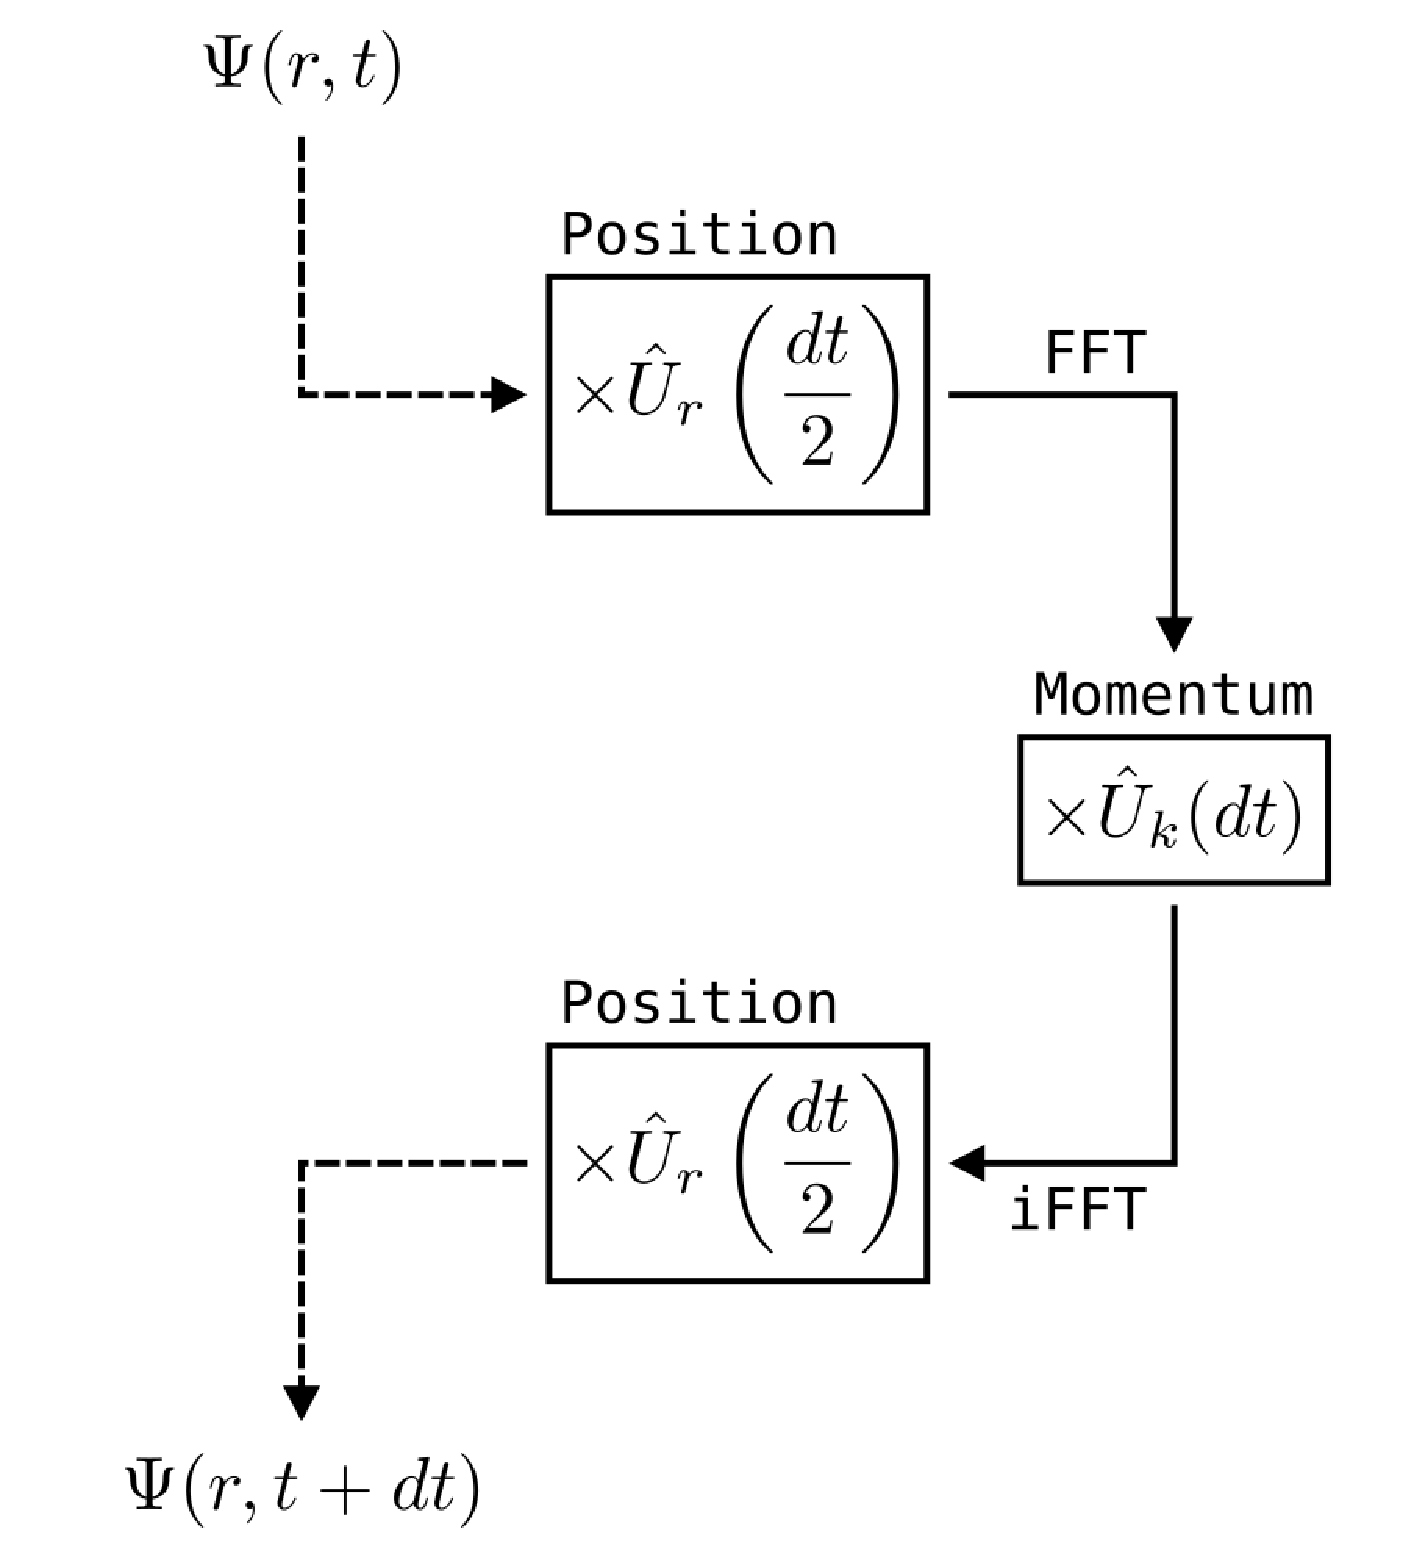
\includegraphics[width=0.5\textwidth]{data/splitop/method/split_op_method.pdf}

\caption{A pictorial representation of the SSFM, created by Julian Schacher~\cite{AAA}.}
\label{fig:method}
\end{figure}

Simply stated, the SSFM splits the Hamiltonian into separate operators and uses a Fourier transform on the wavefunction to ensure that these operators are applied in the appropriate space.
In order to apply the Hamiltonian to the system, we first assume a somewhat general solution to the Schr\"odinger equation,

$$
\Psi(\mathbf{r},t + dt) = \left[e^{-\frac{i\mathcal{\hat{H}}dt}{\hbar}}\right]\Psi(\mathbf{r},t) = \left[e^{-\frac{i(\mathcal{\hat{H}}_v + \mathcal{\hat{H}}_p)dt}{\hbar}}\right]\Psi(\mathbf{r},t).
$$

\noindent If we assume we are simulating our system by a series of small timesteps ($dt$), we can split this operation by using the Baker-Campbell-Housdorff formula \jrs{CN}:

$$
\Psi(\mathbf{r},t+dt) = \left[e^{-\frac{i\mathcal{\hat{H}}_vdt}{\hbar}}e^{-\frac{i\mathcal{\hat{H}}_pdt}{\hbar}}e^{-\frac{[i\hat{H}_r, i\hat{H}_k]dt^2}{2}}\right]\Psi(\mathbf{r},t)
$$

\noindent This accrues a small amount of error ($dt^2$) related to the third term, which is a commutation of the real and momentum-space components of the Hamiltonian, which is a noticeably high;
However, we can decrease the $dt^2$ error to $dt^3$ by performing a half-step in position space before doing a full-step in momentum space, through a process called \textit{Strang Splitting} like so \jrs{CN}:

$$
\Psi(\mathbf{r},t+dt) = \left[e^{-\frac{i\mathcal{\hat{H}}_vdt}{2\hbar}}e^{-\frac{i\mathcal{\hat{H}}_pdt}{\hbar}}e^{-\frac{i\mathcal{\hat{H}}_vdt}{2\hbar}} \right]\Psi(\mathbf{r},t) + \mathcal{O}(dt^3)
$$

\noindent because position and momentum are conjugate domains, we can then address each part of this solution in chunks, first in position space, then in momentum space, then in position space again by using Fourier transforms.
Which looks something like this:

$$
\Psi(\mathbf{r}, t+dt) = \left[\hat{U}_r\left(\frac{dt}{2}\right)\mathcal{F}^{-1}\left[\hat{U}_k(dt) \mathcal{F} \left[\hat{U}_r\left(\frac{dt}{2}\right) \Psi(\mathbf{r},t) \right] \right] \right] + \mathcal{O}(dt^3)
$$

where $\hat{U}_r = e^{-\frac{i\mathcal{\hat{H}}_vdt}{2\hbar}}$, $\hat{U}_k = e^{-\frac{i\mathcal{\hat{H}}_pdt}{\hbar}}$, and $\mathcal{F}$ and $\mathcal{F}^{-1}$ indicate forward and inverse Fourier Transforms.
A flowchart of how we perform this operation can be found in Figure~\ref{fig:method} and is essentially composed of the following steps:

\begin{enumerate}
\item Multiply the wavefunction in real space with the real-space operator.
\item Flip to momentum space with a Fourier transform.
\item Multiply the momentum-space wavefuntion by the momentum-space operator.
\item Flip to position space with an inverse Fourier transform.
\item Repeat 1-4 until satisfied.
\end{enumerate}

The major performance bottleneck for this simulation comes from the Discrete Fourier Transform (DFT) operations, as they are rather costly operations on GPU memory.
In practice, Fast Fourier Transforms (FFTs) are used, often with the Cooley-Tukey method, which was first discovered by Gauss and later contemporized by Cooley and Tukey when they independently discovered it \cite{cooley1965}.
This method is not straightforwardly parallelizable; however, FFT's have become so fundamental to signal processing, that they have been incredibly well-optimized with several libraries, including FFTW~\cite{frigo1998} and CuFFT~\cite{fatica2008} for distributed and GPU calculations, respectively.
We will discuss optimal techniques for using FFTs with the SSFM method in Chapter~\ref{ch:gpue}.

With the method described so far, we can simulate simple quantum systems.
For example, if we guess that our initial wavefunction is gaussian-like and is slightly offset from the center or the trap, this should allow us to see our wavefunction sloshing back and forth in our trap, as shown in Figure~\ref{fig:evolve}(a).

\begin{figure}

\center 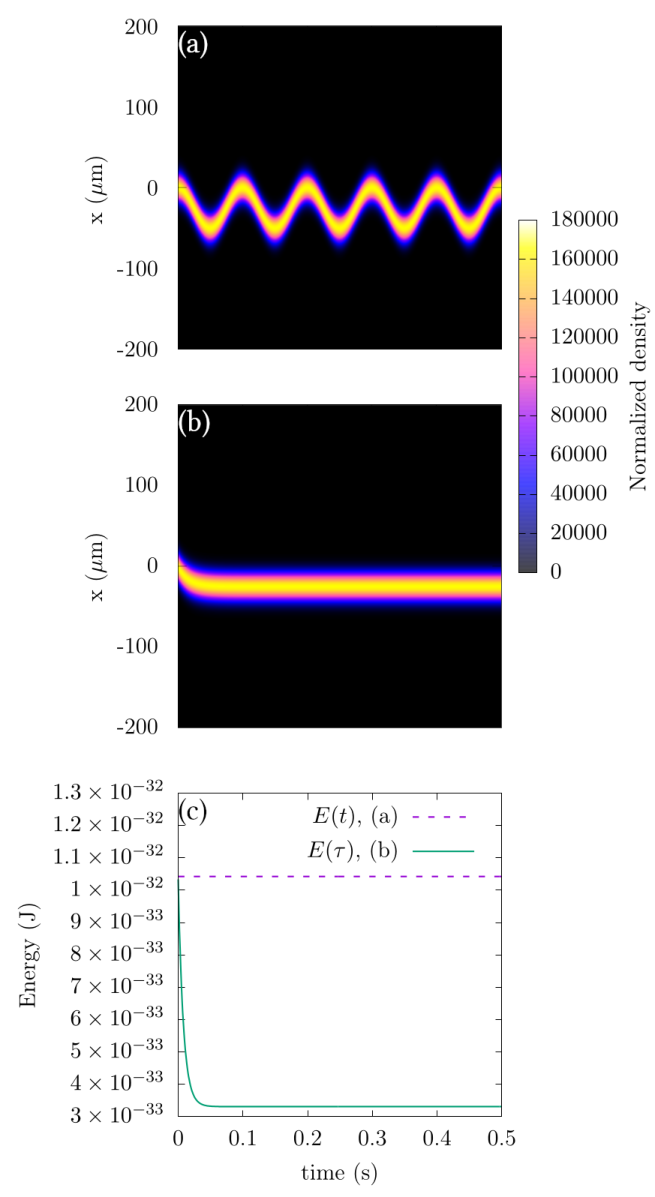
\includegraphics[width=0.6\textwidth]{data/splitop/SHO/SHO_gimp.pdf}

\caption{Evolution of simple harmonic oscillator in real (a), and imaginary (b) time after slightly shifting the trapping potential in the $\hat x$ direction.
In (c), we see the energy as a function of time and show that the energy of the system when evolving in real time remains constant, but in imaginary time it will decay to the known ground-state energy of a simple harmonic oscillator.
The simulated results are from evolution from the split-step Fourier method after 10,000 steps.
Here, we use a Rubidium 87 atom with $\omega_x = 10$Hz on a 256-point grid of size 200 $\mu$m, where the trap has been shifted by 5 $\mu m$.
The wavefunction has been normalized such that $\int_{-\infty}^\infty|\Psi|^2 dx = 1$, which provides arbitrary units.
This simulation was performed with the GPUE codebase \cite{schloss2018}.
\jrs{WIP}}
\label{fig:evolve}
\end{figure}

In addition to this, we can find the lowest energy state of our system with the SSFM by performing a Wick rotation and using $\tau = it$ for the simulation \jrs{CN}.
This changes the solution from sinusoidal to an exponential decay in the energy,

$$
\Psi(\mathbf{r},\tau + d\tau) = \left[e^{-\frac{\mathcal{\hat{H}}d\tau}{\hbar}}\right]\Psi(\mathbf{r},\tau) = \left[e^{-\frac{(E_n d\tau)}{\hbar}}\right]\Psi(\mathbf{r},\tau)
$$

\noindent In this way, by moving our simulation in imaginary time, we will see an exponential decay of the energy and the wavefunction density until we have converged to the ground state.
As we are interested in the dynamics of the quantum system, every step in imaginary time requires a relatively costly renormalization step with

\begin{equation}
    \label{eqn:norm}
    \int_\infty^\infty |\Psi(\mathbf{r},r)|^2 d\mathbf{r} = N,
\end{equation}

\noindent where $N$ is the number of particles in the system.
As this operation requires a summation, it is not well-optimized for GPU hardware; however, it is possible to perform a parallel reduction, which allows for a considerable improvement on massively parallel systems~\cite{harris2007}.
Even so, the normalization is still a slow operation and should be used sparingly.
A simulation of the same system as in Figure~\ref{fig:evolve}(a), but in imaginary time is shown in Figure~\ref{fig:evolve}.
In Figure~\ref{fig:evolve}(c), we see the energy exponentially decaying to the known ground-state energy of a quantum harmonic oscillator of $\frac{1}{2}\hbar\omega$.

Now we will turn our focus to systems to be simulated via the SSFM throughout this work: ultracold atoms.

\section{Introduction to ultracold quantum systems}
\label{sec:intro}

When atomic systems are cooled to temperatures near absolute zero Kelvin, it becomes easier to discern their quantum properties which vary drastically depending on whether the particle is bosonic or fermionic.
Because fermions have half-integer spin, they must obey the Pauli exclusion principle and are constrained to Fermi--Dirac statistics, which means their ground state will be composed of several fermionic pairs.
This creates a \textit{Fermi sea}, where particles fill defined energy levels from the bottom up with two particles per level.
On the other hand, bosons have integer spin and follow Bose--Einstein statistics.
They will condense into a single, macroscopic ground state when cooled~\cite{Einstein1925, Fetter2003}, and
this state of matter is known as a Bose--Einstein Condensate (BEC).
The BEC has the properties of a superfluid, which will be discussed more completely in the following section.

There are notable exceptions to these rules, such as the highly correlated Tonks--Girardeau gas where bosons may act as spinless, non-interacting fermions \cite{Girardeau}.
Though there also exists a regime where interacting fermions can also condense into a BEC-like system~\cite{Nozieres1985, Bulgac2014}, we will not discuss fermionic systems further in this work.
For now, we will focus on BEC systems, but will also discuss Tonks--Girardeau gas systems later in Chapter~\ref{ch:1d}.


\subsection{Bose--Einstein condensation and the Gross--Pitaevskii Equation}

\jrs{DERIVATION NEEDS HELP}
The dynamics of BEC systems can be described by the Gross--Pitaevskii equation, 

\begin{equation}
i \hbar \frac{\partial \Psi(\mathbf{r},t)}{\partial t} = \left(\frac{p^2}{2m} + V_0 + g |\Psi(\mathbf{r},t)|^2 \right)\Psi(\mathbf{r},t)
\label{eqn:GPE}
\end{equation}

\noindent where $\mathbf{r}$ is a position vector, $\Psi(\mathbf{r},t)$ is a many-body quantum wavefunction, $p = -i\hbar\nabla$ is the momentum operator, $V_0$ is the trapping potential, g = $\frac{4\pi\hbar^2 a_s}{m}$ is the interaction strength, $a_s$ is the scattering length of the atomic species, and $m$ is the mass.
The main difference between this equation and the Schr\"odinger equation is the non-linear, interaction term of $g|\Psi|^2$.
When simulating this system, we will find different distribution for the atomic system, known as a Thomas-Fermi distribution, shown in Figure~\ref{fig:TF}

\begin{figure}
\center 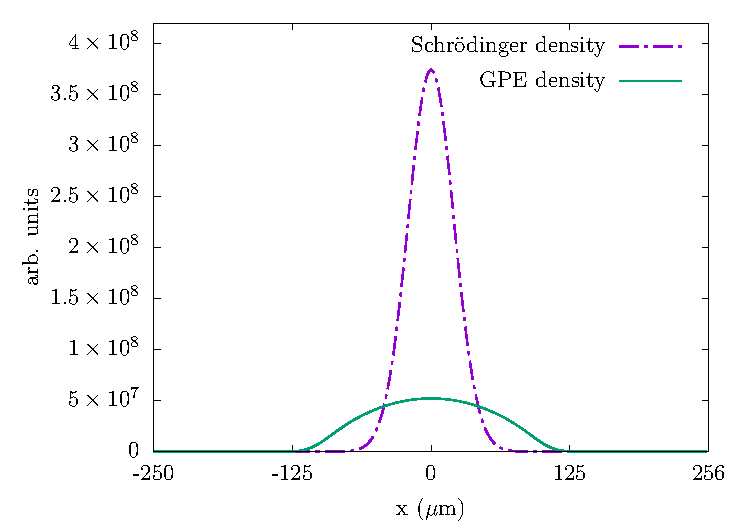
\includegraphics[width = \textwidth]{data/qs/SHO/SHO.pdf}

\caption{Ground state of simple harmonic oscillator for the Schr\"odinger equation (purple, dashed) and the GPE (cyan).
Here, we see that the GPE solution follows a Thomas-Fermi distribution, while the Schr\"odinger equation is Gaussian.
This simulation was performed with GPUE~\cite{schloss2018} for a two-dimensional grid of $256^2$ elements of size $250 \mu m$ with a trapping potential of $\omega_x = \omega_y = 1$, and $1\times 10^6$ particles.}
\label{fig:TF}
\end{figure}


For this section, we will follow a straightforward derivation with the second quantization~\cite{aversa2008}.
As mentioned in Section~\ref{sec:intro}, bosons in a BEC condense into the same (ground) state, meaning we must introduce a many-body Hamiltonian for the system and take inter-particle interactions into account.
For the purposes of this body of work, we will only consider two-body interactions and assume any interactions between three or more atoms to be unlikely and negligible.
We can write the Hamiltonian with two body interactions in the second quantized form as
\begin{equation}
    \mathcal{\hat H} = \int \hat \Psi^\dagger(\mathbf{r})\left[-\frac{\hbar^2}{2m}\nabla^2 + V_0(\mathbf{r}) \right]\hat \Psi(\mathbf{r}) d\mathbf{r} + \frac{1}{2} \int  \hat \Psi^\dagger(\mathbf{r}) \hat \Psi^\dagger(\mathbf{r'}) V(\mathbf{r} - \mathbf{r'})\hat \Psi(\mathbf{r'}) \hat \Psi(\mathbf{r}) d\mathbf{r} d\mathbf{r'}
    \label{eqn:2nd}
\end{equation}
where $\mathbf{r}$ and $\mathbf{r'}$ are the positions of the two colliding particles, $V(\mathbf{r}-\mathbf{r'})$ is the interaction potential, and $\hat \Psi^\dagger(\mathbf{r})$ and $\hat \Psi(\mathbf{r})$ are the creation and annihilation operators that follow the commutation relations,
\begin{align}
 [\hat \Psi(\mathbf{r}),\hat \Psi^\dagger(\mathbf{r})] &= \delta(\mathbf{r} - \mathbf{r'}) \\
 [\hat \Psi^\dagger(\mathbf{r}),\hat \Psi^\dagger(\mathbf{r})] &= 0 \\
 [\hat \Psi(\mathbf{r}),\hat \Psi(\mathbf{r})] &= 0.
\end{align}

In the case of a BEC at $T\approx0$, we may perform a Bogoliubov expansion~\cite{Bogoliubov1947, Dalfovo1999}
\begin{equation}
    \hat \Psi (\mathbf{r}, t) = \Phi(\mathbf{r},t) + \delta \hat \Phi(\mathbf{r},t)
\label{eqn:bog}
\end{equation}
where $\Phi(\mathbf{r},t) \equiv \langle \hat \Psi(\mathbf{r},t) \rangle$ is the wavefunction of the condensate known as the \textit{order parameter} and $\delta \hat \Phi(\mathbf{r},t)$ represents fluctuations of the BEC system.
In a BEC, the condensate density is defined as
\begin{equation}
    n(\mathbf{r},t) = |\Phi(\mathbf{r},t)|^2.
\end{equation}

Now we may use the Heisenberg equation of motion
\begin{equation}
    i\hbar \frac{\partial}{\partial t}\hat \Psi(\mathbf{r},t) = [\hat \Psi, \hat H]
\end{equation}
    to determine the time evolution of the field operator $\hat \Psi(\mathbf{r},t)$ as
\begin{equation}
    \frac{\partial}{\partial t}\hat \Psi(\mathbf{r},t) = \frac{1}{i\hbar}\left[-\frac{\hbar^2}{2m}\nabla^2 + V_0(\mathbf{r}) + \int d\mathbf{r'} \hat \Psi^\dagger(\mathbf{r'}, t)V(\mathbf{r'} -\mathbf{r})\hat \Psi(\mathbf{r'},t)\right]\hat \Psi(\mathbf{r},t),
\end{equation}
which follows from Equation~\eqref{eqn:2nd} after integrating over $\mathbf{r}$. 
Now we must apply a few approximations for the BEC:
\begin{enumerate}
    \item In the Bogoliubov expansion, Equation~\eqref{eqn:bog}, we assume that $\delta \hat \Phi(\mathbf{r},t)$ is small at $T = 0\text{K}$, and thus $\hat \Psi(\mathbf{r},t) \approx \Phi(\mathbf{r},t)$. 
    \item Two bosons will only interact with a contact potential of the form
    \begin{equation}
        V(\mathbf{r'}-\mathbf{r}) = g\delta(\mathbf{r'} - \mathbf{r}),
    \end{equation}
    which has a strength given by
    \begin{equation}
        g \equiv \frac{4 \pi \hbar^2 a_s}{m},
    \end{equation}
    where $a_s$ is the species and state-dependent s-wave scattering length.
    %\item The bose gas is dilute and the inter-particle spacing is much larger than $a_s$.
\end{enumerate}

With these approximations, we may write the time-dependent Schr\"odinger equation as
\begin{equation}
    i\hbar \frac{\partial}{\partial t}\Phi(\mathbf{r},t) = \left( - \frac{\hbar^2}{2m} \nabla^2 + V_0(\mathbf{r}) + g |\Phi(\mathbf{r},t)|^2\right)\Phi(\mathbf{r},t).
\end{equation}
This equation is known as the nonlinear Schr\"odinger equation due to the presence of the $|\Phi(\mathbf{r},t)|^2$ term.
In the BEC community, the equation is usually called the Gross-Pitaevskii equation (GPE).
When written in the time-independent form it determines the chemical potential $\mu$ of the condensate system~\cite{Gross1961, Pitaevskii1961}
\begin{equation}
    \mu\Phi(\mathbf{r}) = \left( - \frac{\hbar^2}{2m} \nabla^2 + V_0(\mathbf{r}) + g |\Phi(\mathbf{r})|^2\right)\Phi(\mathbf{r},t).
    \label{eqn:GP}
\end{equation}

This equation allows us to determine the full dynamics of a BEC system and the numerical solutions will be discussed in subsequent chapters.
Similar derivations of the GPE can be found in many introductory texts on BEC physics, such as~\cite{Fetter2003, Pethick2002, Fetter2009}.

It is important to note that a BEC acts like a superfluid, which is a state of matter that is similar to a classical fluid without viscosity.
This means that once a superfluid is set in motion, there is no retarding force to keep it from flowing.
There are a few known systems in which superfluidity can exist, such as $^4$He (sometimes called Helium II when in its superfluid phase)~\cite{Allen1938}, neutron stars~\cite{Migdal1960}, or BEC systems~\cite{Einstein1925, Anderson1995}.
BEC systems are generally cleaner experimental systems to create, as they do not have a classical fluid fraction, like $^4$He.
As stated, we will focus on BEC systems in this work, but it is important to note that any results shown for BEC systems may have applications beyond cold, atomic physics.

\section{Superfluid systems and vortex dynamics}

Though there are many interesting differences between classical fluids and superfluids, we will focus here on vortex dynamics.
By rotating a fluid, it is possible to create a vortex around the axis of rotation; however, because of the viscosity of a classical fluid, the vortex will begin to shrink and eventually disappear without constant driving.
In a superfluid, this is not necessarily the case.

In addition, due to the quantization of angular momentum in quantum mechanics, the vorticity in a superfluid is also quantized with the circulation defined as~\cite{Pethick2002},
\begin{equation}
\Gamma = \oint\mathbf{v} \cdot d \mathbf{l} = 2\pi \frac{\ell \hbar}{m},
\label{Eq:phase}
\end{equation}
where $\ell$ is an integer value known as the phase winding, and $m$ is the mass of the atomic species.
In this case, the velocity is
\begin{equation}
v = \frac{\hbar}{m}\mathbf{\nabla}\phi,
\end{equation}
with $\phi$ as the phase.
Every singly-charged vortex in a BEC will have a $2\pi$ phase winding, and an example simulation with one vortex and its corresponding phase can be seen in Figure~\ref{fig:rot} (a and b).

\begin{figure}

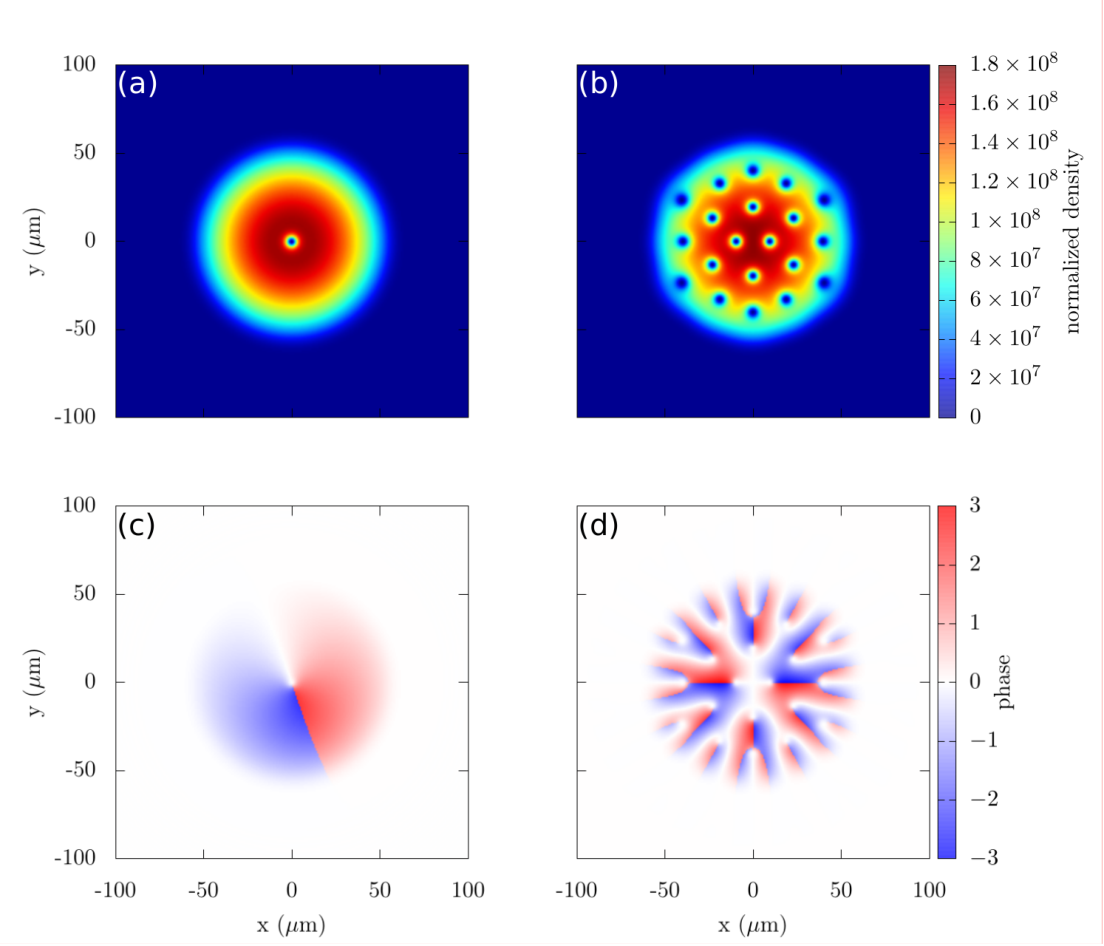
\includegraphics[width=\textwidth]{data/splitop/rot/WIP.pdf}

\caption{
Simulation of rotation with a single vortex (a, b) and a vortex lattice (c, d).
The wavefunction density is shown in a and c, while the corresponding phase is shown in b and d.
A rotation of $\Omega = 0.35\omega_x$ was used for a and b, while a rotation of $\Omega = 0.99\omega_x$ was used for c and d.
Here, we use a Rubidium 87 atom with $\omega_x = 2\pi$Hz on a 512-point grid of size 200 $\mu$m.
This simulation was performed with the GPUE codebase \cite{schloss2018}, and the phase plost are created by multiplying the phase by the wavefunction density to remove anomalous noise beyond the BEC boundary.
\jrs{WIP}}
\label{fig:rot}
\end{figure}

Because the energy $E \propto \ell^2$ and $\ell$ is an integer value, as a superfluid is spun faster, a vortex will not grow or shrink in size, but multiple vortices will spawn instead~\cite{Pethick2002}.
In other words, it is energetically favorable for two vortices of smaller angular mementum to form instead of a single vortex with a large amount of angular momentum.
Large amounts of angular momentum will therefore lead to many vortices, which will arrange themselves in a triangular lattice structure known as an Abrikosov lattice~\cite{Abrikosov1957, Fetter2001}.
This behaviour is identical to that of Type II superconductors under the effects of a magnetic field, where the size of each vortex is described by a physical property known as the healing length.
An example of this vortex lattice and its phase can be seen in Figure~\ref{fig:rot} (c and d).

The three-dimensional properties of vortices in superfluid systems are also peculiar in their behaviour when compared to their classical counterparts.
Superfluid vortices must either end at the end of the condensate or reconnect in the form of vortex rings or other, more complicated vortex structures~\cite{Reichl2013}.
Because the circulation around superfluid vortices is quantized, when two vortices approach each other with different velocity fields, they may reconnect into smaller, more energetically favorable vortex structures.
During this reconnection, the abrupt change in energy will create a sound wave at the reconnection site~\cite{Feynman1955}.

Three dimensional vortex structures of non-trivial topology have been notoriously difficult to generate in a controllable way experimentally, but we will discuss an experimentally viable method to generate, control, and detect vortex ring-like structures in superfluid BEC systems in Chapter~\ref{ch:vortex_states}.
There are currently three primary process to controllably generate vortex structres in superfluid systems: rotation, phase imprinting, and artificial magnetic fields.

\subsection{Rotation}

\label{sec:rot}
As mentioned, rotation of a BEC system will provide vortex lines that follow the axis of rotation and start and end on the BEC boundary.
Examples of vortex lines in two-dimensions can be seen in Figure~\ref{fig:rot}.
To simulate the effects of rotation, we simply need to append the angular momentum operator $L_z = -i\hbar(xp_y - yp_x)$ to the GPE:

\begin{equation}
i \hbar \frac{\partial \Psi(\mathbf{r},t)}{\partial t} = \left(\frac{p^2}{2m} + V_0 + g |\Psi(\mathbf{r},t)|^2 -\Omega L_z \right)\Psi(\mathbf{r},t),
\end{equation}

\noindent where $\Omega$ is the rotation frequency. 
In order to generate a vortex via rotation, we must rotate faster than the critical velocity of $\Omega_c \simeq 0.3 \omega_x$, where $\omega_x$ is the trapping frequency.
In addition, if the rotation frequecy is greater than the trapping frequency, the atoms will no longer be bound by the trap due to centripetal forces.
As such, finding the appropriate rotation frequency for creating vortex lattices in BEC systems is a precarious balancing act.
Largescale vortex lattices have been generated both experimentally and theoretically, with the largest vortex lattices being generated with $\Omega \approx \omega_x$ \cite{o2016, o2016topo, abo2001, Schweikhard2004}.

In this work, we use rotation in a similar way; however, we will later introduce articifial magnetic fields, which is a broader framework that encompases rotation and will be used in all our simulations moving forward.
We will discuss this in more detail in Section~\ref{sec:implementation}.

\subsection{Phase imprinting}

Phase imprinting is a powerful tool to allow for the generation of various structures in atomic systems \cite{kumar2018, moulder2012, burger1999, denschlag2000}.
In principle, this technique relies on imprinting a $2\pi$ phase winding along the vortex line researchers wish to create.
Experimentally, phase imprinting can be done in a number of ways.
As an example, the phase could be imprinted with a Raman two-photon process to transfer orbital angular momentum to atoms from a Laguerre--Gaussian beam \cite{moulder2012, ryu2007}.
Another method is through pulsing a spatially dependent potential for a short time when compared to the trapping frequency, which will imprint the potential onto the phase of the system~\cite{kasevich1991} and can be used to generate a soliton~\cite{denschlag2000}, vortex~\cite{gajda1999}, or other states with quantized circulation~\cite{kumar2018}.
In both of these methods, it is possible to create vortex structures that are more complex than simple vortex lines.
Phase imprinting has also been used in theoretical studies to create a defect in a large vortex lattice by flipping the phase (and therefore rotation direction) of a selected vortex by imprinting a $-4\pi$ phase at the vortex's location~\cite{o2016topo}.
Note that if a phase greater than $|2\pi|$ is imprinted onto the system, the vortices are likely to decay into vortices of $|2\pi|$ phase~\cite{shin2004}.

For the purposes of this work, we will only consider imprinting vortex lines with this method by apply phase imprinting operations to our condensate, such that

\begin{equation}
\Psi_{IMP}(x,y,t) = |\Psi(x,y,t)|e^{i(\theta(x,y,t) + \theta_{IMP}(x,y))}
\end{equation}

\noindent where $\Psi_{IMP}(x,y,t)$ is the quantum wavefunction after phase imprinting, $\theta(x,y,t)$ is the phase of the quantum system, and $\theta(x,y) = \text{arctan}(y-y_0, x-x_0)$ centers the phase profile at position $(x_0, y_0)$.
This method allows us to apply a phase mask to any location in the transverse plane and will be applied further in Chapter~\ref{ch:2d}.

Phase imprinting has allowed for the generation of many interesting vortex topologies in theoretical and experimental studies~\cite{white2014, maucher2016}; however, it is a destructive process that does not create eigenstates of the system.
As such, it is not as useful for engineering stable vortex structures, but is instead useful for dynamical studies, such as those found in Chapter~\ref{ch:2d}.

\subsection{Artificial magnetic fields}
\label{sec:gauge}

Magnetic fields are capable of generating rotational effects in charged systems through the Lorentz force, $F_l = q(\mathbf{E} + \mathbf{v} \times \mathbf{B})$, where $q$ is the charge of the system, $\mathbf{E}$ is the electric field, $\mathbf{B}$ is the magnetic field, and $\mathbf{v}$ is the velocity of the particle.
This effect will allow for the creation of vortices in type II superconductors; however, it is not directly applicable to BEC systems because BECs are typically weakly interacting and composed of neutral atoms, which do not have charge.
Even so, it is possible to generate artificial magnetic fields with similar effects, and these artificial magnetic fields have even been shown to create vortices experimentally~\cite{Lin2009}.
In addition, artificial magnetic fields create a broader framework that encompassses rotational effects previously shown in Section~\ref{sec:rot}, and we will use this framework for the remainder of this work.
As such, a detailed introduction, similar to that given by Dalibard in~\cite{Dalibard2015}, will be presented below.

If written in the Hamiltonian formalism, the Lorentz force law becomes

\begin{equation}
\mathcal{\hat{H}} = \frac{(\mathbf{\hat p} - q\mathbf{A}(\mathbf{r}))^2}{2m}
\end{equation}

\noindent where $\mathbf{A}$ is a vector potential such that $\mathbf{B} = \nabla \times \mathbf{A}$ and $q$ is the charge of the particle.
Because cold atoms are neutral, we must find ways to simulate the effects of magnetic fields instead of using magnetic fields themselves.

Firstly, let us describe how rotation can be considered to be an artificial vector potential and thus generate vortex structures in BEC systems.
Imagine a plane rotating with an angular velocity $\Omega$ around the $z$-axis ($\mathbf{\Omega} = \Omega \hat z$). 
In this case, the Coriolis force is defined as
\begin{equation}
\mathbf{F}_{\text{Coriolis}} = 2m \mathbf{v} \times \mathbf{\Omega},
\end{equation}
which is formally similar to the Lorentz force law.
By applying the transformation $\hat H = \hat H_0 - \Omega \hat L_z$, where $\hat L_z = x\partial_y - y\partial_x$, we find~\cite{Bhat2008}
\begin{equation}
\begin{split}
\hat H &= -\frac{\hbar^2}{2m}\nabla^2 + \frac 1 2 m \omega^2(x^2 + y^2) - \frac{\hbar \Omega}{i}(x\partial_y - y\partial_x) \\
 &= \frac{1}{2m}\left(\frac{\hbar}{i}\nabla - m(\mathbf{\Omega} \times \mathbf{r})\right)^2 + \frac m 2 \left( \omega^2 - \Omega^2 \right)r^2 \\
 &= \frac{(\hat{\mathbf{p}}-m\mathbf{A}(\mathbf{r}))^2}{2m}+ V_0(\mathbf{r}),
\end{split}
\end{equation}
where $\omega$ is the trapping frequency for a symmetric two-dimensional harmonic trap, $\mathbf{A} \equiv \mathbf{\Omega} \times \mathbf{r}$, and $V_0 = m/2 \left( \omega^2 - \Omega^2 \right)r^2$.
The final form is similar to that of the Lorentz force law and coincides with an effective magnetic field of $2 \mathbf \Omega \propto \mathbf B$.
In this way, we may recreate the rotation expected from the Lorentz force law in a cold atomic system with an artificial magnetic field~\cite{Peshkin1989, Madison2000, Abo-Shaeer2001}.

Here, it becomes more obvious why it is impossible to rotate a system when $\Omega > \omega_x$, as the potential term $V_0$ becomes negative at that point.
Artificial magnetic fields provide a powerful tool to researchers who wish to generate and control complex vortex structures, and because of this, it is worth discussing them in further detail.
Important implementation details for how to use artificial magnetic fields with the SSFM will be noted in Section~\ref{sec:implementation}.

\subsubsection{Geometric Gauge Fields}
\label{sec:geom}

As we have already described how rotation can act as an artificial Lorentz force, we now turn our attention towards methods that might allow us to generate more general rotational effects and vortex structures.
In particular, we will discuss the adiabatic motion of free atoms undergoing geometric phase transformations through the Berry phase. 
For this, we assume that our system has an external parameter $\lambda$ such that
\begin{equation}
\hat H(\lambda) \ket{\psi_n(\lambda)} = E_n(\lambda)\ket{\psi_n(\lambda)},
\end{equation}
where the set of eigenstates $\left\{ \ket{\psi_n(\lambda)} \right\}$ allow us to define the time evolution of our system such that
\begin{equation}
\ket{\psi(t)} = \sum_n c_n(t) \ket{\psi_n(\lambda(t))},
\end{equation}
and we consider $\lambda$ to evolve slowly with time. If we consider the system to begin with
\begin{equation}
c_l(0) = 1,
\qquad
c_n(0) = 0, 
\qquad
\text{for all } n\neq l
\end{equation}
the state of the system is proportional to $\ket{\psi_l(\lambda(t))}$.
In this case, $c_l(t)$ is determined by the equation
\begin{equation}
i \hbar \dot{c}_l =  [E_l(t) - \dot{\lambda} \cdot \mathbf{A}_l(\lambda)]c_l,
\label{Bcnx-1}
\end{equation}
where 
\begin{equation}
\mathbf{A}_l(\lambda) = i \hbar \braket{\psi_l|\nabla\psi_l}.
\label{eqn:Bcnx}
\end{equation}
This quantity is called the Berry connection, which is considered a vector potential, such that we can define a new artificial magnetic field, the Berry curvature as
\begin{equation}
\mathbf{B}_l = \mathbf{\nabla} \times \mathbf{A}_l.
\label{eqn:BC}
\end{equation}

Now imagine that the $\lambda$ parameter follows the closed contour $C$ such that $\lambda(T) = \lambda(0)$. 
By integrating Equation~\eqref{Bcnx-1} above, we find
\begin{equation}
c_l(t) = e^{i \Phi_{\text{dyn}}(t)}e^{i\Phi_{\text B}(T)}c_l(0),
\label{eqn:c}
\end{equation}
where
\begin{equation}
\begin{split}
\Phi_{\text{dyn}}(T) &= - \frac{1}{\hbar}\int_0^TE_l(t)dt \\
\Phi_{\text{Berry}} (T)&= \frac{1}{\hbar} \int_0 ^T \dot{\lambda} \cdot \mathbf{A}_l(\lambda)dt = \frac{1}{\hbar}\oint\mathbf{A}_l(\lambda) \cdot d\lambda
\end{split}
\end{equation}
In this case $\Phi_{\text{Berry}}$ is called the Berry phase and it only depends on the motion path of $\lambda$. 
It should be mentioned that both of the exponential terms in Equation~\eqref{eqn:c} are gauge invariant and thus remain unchanged when $\ket{\psi_n(\lambda)}$ is multiplied by a phase factor.
This phase allows us to transfer angular momentum into our BEC and generate a vortex geometry like those formed in the 2009 experiment by Lin~\textit{et~al.}~\cite{Lin2009}.
As a note, the vortex structures generated in this way follow the magnetic fields lines, thus providing the capability to generate complex vortex structures beyond vortex lines.
Outside of rotation, another method to generate these gauge fields in an experimentally realizable way will be described in Chapter~\ref{ch:vortex_states}, but for now we should discuss how these fields can be implemented in the SSFM, with an emphasis on their effects for superfluid simulations.

\section{Modifications to the SSFM for superfluid vortex simulations}
\label{sec:implementation}

In order to simulate the effects of artificial magnetic fields on BEC systems, we must slightly modify the Hamiltonian, like so:

\begin{equation}
\mathcal{\hat H} = \frac{(p-m\mathbf{A})^2}{2m} + V_0 + g|\Psi(\mathbf{r},t)|^2
\end{equation}

Where $\mathbf{A}$ is an artificial vector potential of various forms.
As a note, some texts absorb the mass term into the artificial vector potential, but here we are stating it explicitly for convenience.
When expanded, we note that the gauge field has a component in position space, $\frac{m\mathbf{A}^2}{2}$, which couples with the trapping potential, and another component that is partially in both position and momentum space, $p\mathbf{A}$.

Firstly, let us discuss the component purely in position space.
Here, we see that it is important to properly balance the trapping potential and the artificial vector potential when simulating BEC systems with rotation or other artificial vector potentials, otherwise, the trapping geometry will become warped.
As mentioned in Section~\ref{sec:rot}, this is effectively balanced by the centripetal force; however, 
in the case of arbitrarily chosen vector potentials, this can create rather unusual wavefunction geometries, as shown in Figure~\ref{fig:V_change} for a gaussian $\mathbf{A_x}$ and $\mathbf{A_y}$.
Though we might be able to balance this warping with a centripetal force tailored to the gauge fields we introduce, we did not consider this for the purposes of this work.

\begin{figure}

\begin{centering}
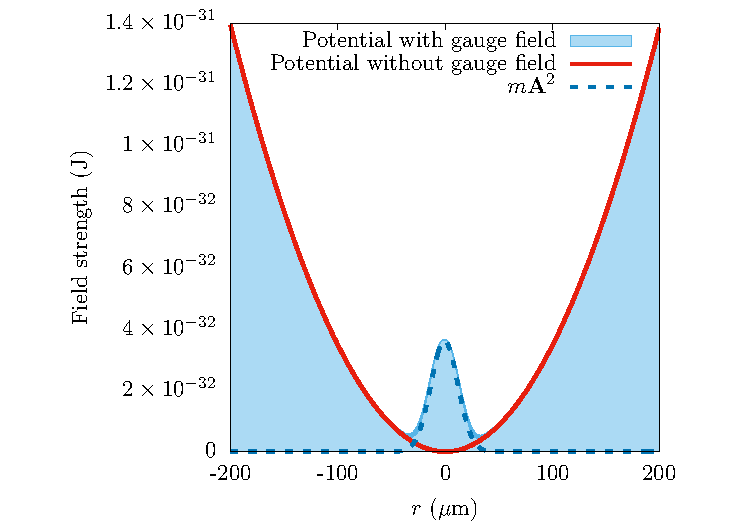
\includegraphics[width=0.48\textwidth]{data/splitop/gauge/check.pdf}
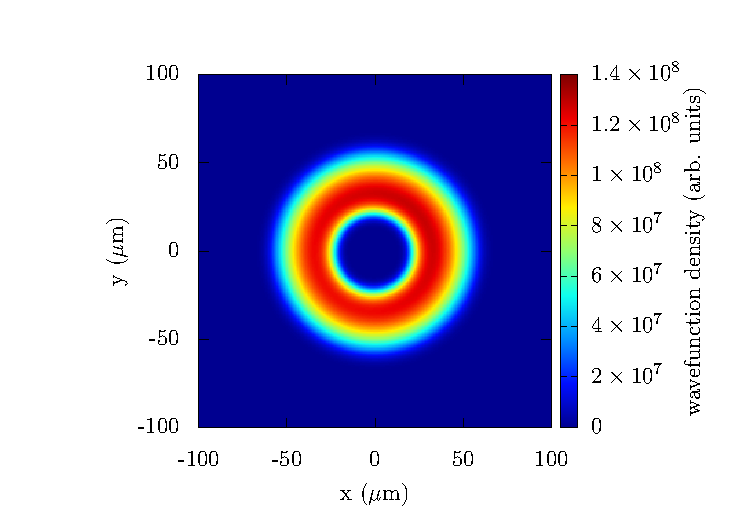
\includegraphics[width=0.48\textwidth]{data/splitop/gauge/density.pdf}
\end{centering}

\caption{
Simulation of GPE with an arbitrarily chosen gaussian artificial vector potential.
For this simulation, we have removed the $pA$ term to focus on the warped potential, itself.
This simulation was performed with the GPUE codebase \cite{schloss2018}.
\jrs{WIP}}
\label{fig:V_change}
\end{figure}

The components of the artificial vector potential that are partially in position and momentum space are somewhat difficult to consider numerically.
As they reside in both spaces, it is required to perform a one-dimensional FFT acros $n$-dimensional data.
This means that if we have three operators, $p\mathbf{A}_x \hat x$, $p\mathbf{A}_y \hat y$, and $p\mathbf{A}_z \hat z$, we will need to perform an FFT on our wavefunction in the $\hat x$, $\hat y$, and $\hat z$ dimensions, respectively, before applying the operators through element-wise multiplication. 
As discussed in Chapter~\ref{ch:gpu}, this has significant performance penalties if we do not consider appropriate memory coalescence.
This also requires the usage of more intricate FFT plans for the FFTW or CuFFT libraries, which are non-trivial for three-dimensional simulations.
In particular, it should be noted that more optimal FFT schemes require transposing the data to ensure memory coalescence for each of these FFT operations.
In fact, a tranpose of this nature would also made the global FFT operations faster for the SSFM without rotation.
As such, we have also designed an in-place, three-dimensional, distributed transpose for multi-GPU SSFM calculations.
Direct implementation details will be further described in Chapter~\ref{ch:gpu}.
